\section{Convolution and Filtering}

Convolution and filtering are some of the most basic operations of image processing. 


\subsection{Filtering}

Image filtering is the process of modifying pixels in an image base on some function of a local neighborhood of the pixel.

\subsubsection{Linear Shift-Invariant Filtering}

Linear lhift-invariant filtering means using linear combinations of neighbors and doing the same for each pixel (shift-invariant). These filters are often used for low-level image processing, smoothing / noise reduction, sharpening and feature detection. Linear operations can be written as:
$$I'(x,y) = \sum_{(i,j) \in N(x,y)} K(x,y; i, j) I(x,y)$$

Here $I$ is the input image, $I'$ the output image, $K$ is the kernel and $N$ is the neighborhood. Operations are shift-invariant if $K$ does not depend on $(x,y)$.


\subsection{Correlation}

Correlation, e.g. template matching:

\begin{center}
	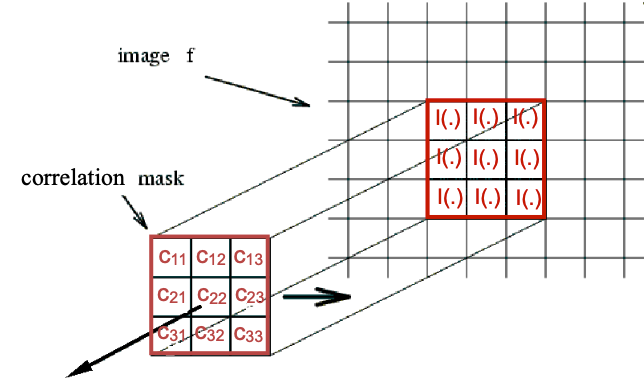
\includegraphics[width=0.9\linewidth]{correlation.png}
\end{center}
$$I' = K \circ I, \quad I'(x,y) = \sum_{(i,j) \in N(x,y)} K(i, j) I(x + i, y + j)$$

Correlation takes an input image and a weight mask, then each pixel gets "replaced" by the weighted sum of its neighborhood. This can be described as taking multiple input location and writing one output location.


\subsection{Convolution}

Convolution, e.g. point spread function:

\begin{center}
	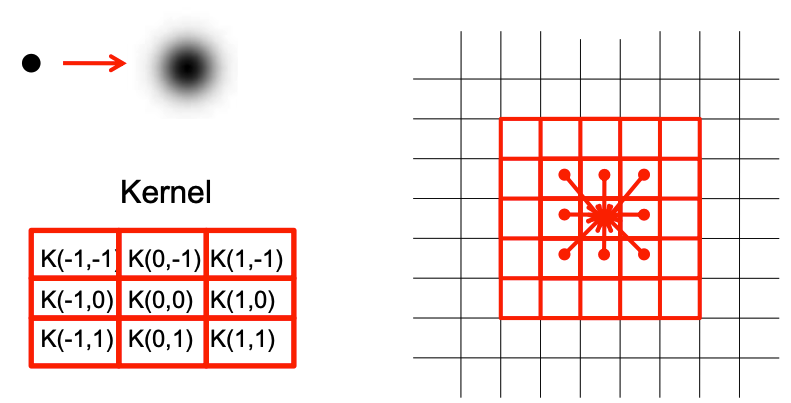
\includegraphics[width=0.9\linewidth]{convolution.png}
\end{center}
$$I' = K * I, \quad I'(x,y) = \sum_{(i,j) \in N(x,y)} K(i, j) I(x - i, y - j)$$

This is similar to the correlation, but \textbf{the kernel is reversed}. This can be described as taking one input location and writing multiple output location, the opposite of the correlation. By default we use convolution for filtering. An example for a kernel would be:
$$ K = 
\begin{bmatrix}
    0 & 0 & 0\\
    0 & 2 & 0\\
    0 & 0 & 0
\end{bmatrix}
 -
\frac{1}{9}
\begin{bmatrix}
   1 & 1 & 1\\
   1 & 1 & 1\\
   1 & 1 & 1
\end{bmatrix}
$$

This kernel is used for sharpening by accentuating differences with the local average. Another example would be:
$$ K = 
\begin{bmatrix}
    -1 & 0 & 1\\
    -2 & 0 & 2\\
    -1 & 0 & 1
\end{bmatrix}
$$

This kernel looks for differences in the horizontal direction, this corresponds to finding vertical edges.

\subsubsection{What about the Edges?}

If we apply our filters to images, we need to \textbf{deal with the edges separately}. This is due to our window falling off the edge of the image. There are different techniques to deal with this problem:
\begin{itemize}
	\item Extend the image with black border
	\item Wrap the kernel around the edges
	\item Copy out the edge
	\item Mirror the image at the edge
	\item Vary filter near the edge
\end{itemize}

\subsubsection{Separable Kernels}

A kernel is separable, if it can be written as $K(m, n) = f(m) g(n)$. This means that the kernel can be separated into a function for the first coordinate and another for the second coordinate. If this is the case we can apply the separated functions individually to the image.

\subsubsection{Gaussian Kernel}

The idea of the \textbf{Gaussian Kernel} is to weight the contributions of neighboring pixels by nearness.

\begin{center}
	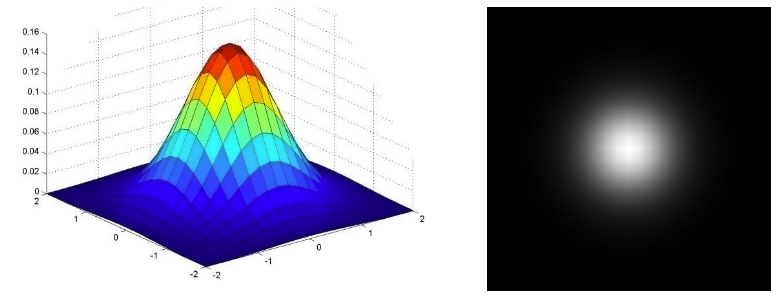
\includegraphics[width=0.9\linewidth]{gaussian_kernel.png}
\end{center}
$$G_\sigma = \frac{1}{2 \pi \sigma^2}^{- \frac{(x^2 + y^2)}{2 \sigma^2}}$$

We can use the Gaussian Kernel for image smoothing, the best part being that the kernel is separable. The actual amount of smoothing depends on $\sigma$ and the window size. \medskip

If we repeatedly apply the Gaussian filter, we produce the scale space of an image.

\subsubsection{High-Pass Filters}

High-pass filters are used to detect areas of the image where a lot is happening (high frequencies). Examples for these are the Laplacian operator $K$ or the high-pass filter $K'$:
$$ K = 
\begin{bmatrix}
    0 & 1 & 0\\
    1 & -1 & 1\\
    0 & 1 & 0
\end{bmatrix}
\qquad
K' =
\begin{bmatrix}
    -1 & -1 & -1\\
    -1 & 8 & -1\\
    -1 & -1 & -1
\end{bmatrix}
$$

High-pass filters can be used to perform image sharpening $I' = I + \alpha |K * I|$.


